\begin{figure}[htbp]
      \centering
    \scriptsize
        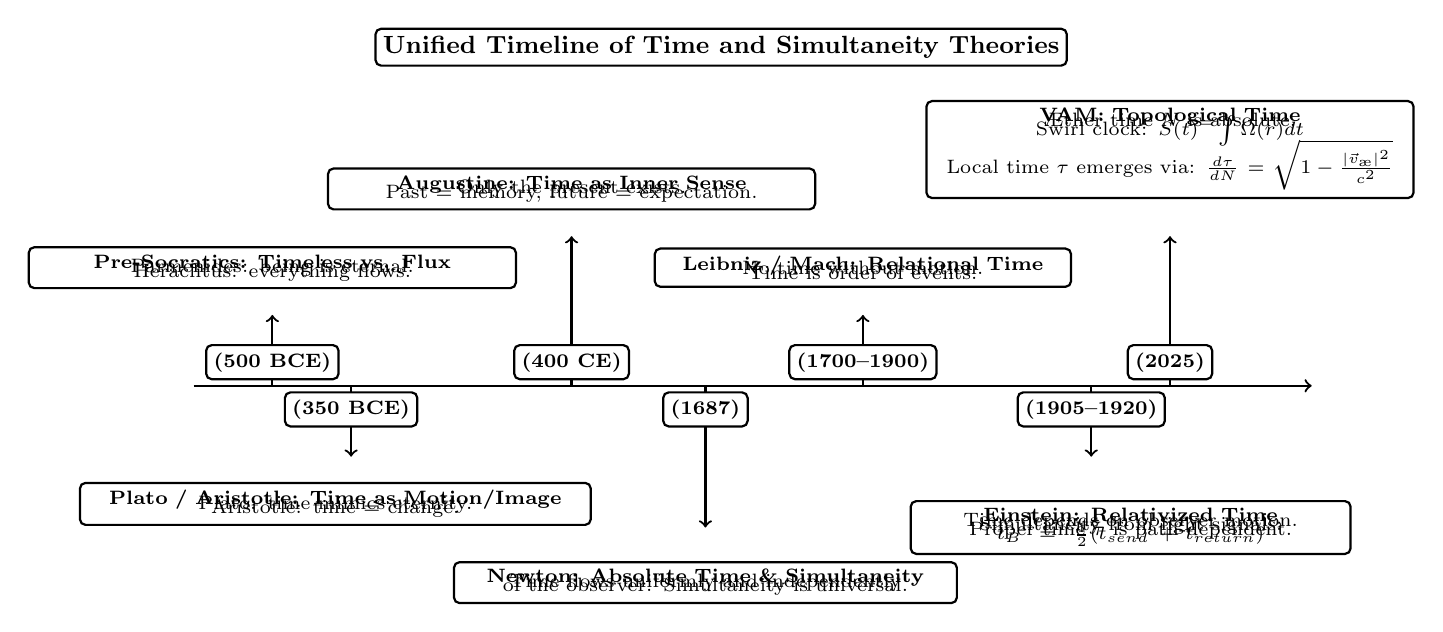
\begin{tikzpicture}
        \scriptsize
        % Timeline base
        \draw[->, thick] (-1,0) -- (13.2,0);

        % Arrows above timeline (short, as requested)
        \draw[->, thick] (0,0) -- (0,0.9);       % Pre-Socratics
        \draw[->, thick] (3.8,0) -- (3.8,1.9);   % Augustine
        \draw[->, thick] (7.5,0) -- (7.5,0.9);   % Einstein
        \draw[->, thick] (11.4,0) -- (11.4,1.9); % VAM

        % Arrows below timeline (short, as requested)
        \draw[->, thick] (1.0,0) -- (1.0,-0.9);     % Plato/Aristotle
        \draw[->, thick] (5.5,0) -- (5.5,-1.8);     % Newton
        \draw[->, thick] (10.4,0) -- (10.4,-0.9);     % Leibniz/Mach

            %--- Root title cards (above timeline) ---
        \node[draw, thick, rounded corners=2pt, fill=white, align=center, font=\bfseries ] at (0, .3)   {(500 BCE)};
        \node[draw, thick, rounded corners=2pt, fill=white, align=center, font=\bfseries ] at (3.8, .3) {(400 CE)};
        \node[draw, thick, rounded corners=2pt, fill=white, align=center, font=\bfseries ] at (7.5, .3) {(1700--1900)};
        \node[draw, thick, rounded corners=2pt, fill=white, align=center, font=\bfseries ] at (11.4, .3){(2025)};

        %--- Root title cards (below timeline) ---
        \node[draw, thick, rounded corners=2pt, fill=white, align=center, font=\bfseries ] at (1.0,- .3) {(350 BCE)};
        \node[draw, thick, rounded corners=2pt, fill=white, align=center, font=\bfseries ] at (5.5,- .3) {(1687)};
        \node[draw, thick, rounded corners=2pt, fill=white, align=center, font=\bfseries ] at (10.4,- .3) {(1905--1920)};

            % Timeline label
        \node[draw, thick, fill=white, rounded corners=2pt, font=\small] at (5.7,4.3) {\textbf{Unified Timeline of Time and Simultaneity Theories}};

        % --- Pre-Socratics ---
        \node[draw, rounded corners=2pt, thick, align=center, fill=white, text width=6cm] at (0,1.5) {
        \textbf{Pre-Socratics: Timeless vs. Flux} \\[-0.8em]
        Parmenides: being is eternal. \\[-0.8em]
        Heraclitus: everything flows.
        };

        % --- Augustine ---
        \node[draw, rounded corners=2pt, thick, align=center, fill=white, text width=6cm] at (3.8,2.5) {
        \textbf{Augustine: Time as Inner Sense} \\[-0.8em]
        Only the present exists. \\[-0.8em]
        Past = memory, future = expectation.
        };

        % --- Leibniz / Mach ---
        \node[draw, rounded corners=2pt, thick, align=center, fill=white, text width=5.1cm] at (7.5,1.5) {
        \textbf{Leibniz / Mach: Relational Time} \\[-0.8em]
        No time without motion. \\[-0.8em]
        Time is order of events.
        };
        % --- VAM (modern) ---
        \node[draw, rounded corners=2pt, thick, align=center, fill=white, text width=6.0cm] at (11.4,3.0) {
        \textbf{VAM: Topological Time} \\[-0.8em]
        Æther time $N$ is absolute. \\[-0.6em]
        Swirl clock: $S(t)^\circlearrowleft = \int \Omega(r) dt$ \\[-0.4em]
        Local time $\tau$ emerges via: $ \frac{d\tau}{dN} = \sqrt{1 - \frac{|\vec{v}_\text{\ae}|^2}{c^2}}$

        };


        % --- Plato / Aristotle ---
        \node[draw, rounded corners=2pt, thick, align=center, fill=white, text width=6.3cm] at (0.8,-1.5) {
        \textbf{Plato / Aristotle: Time as Motion/Image} \\[-0.8em]
        Plato: time mimics eternity. \\[-0.8em]
        Aristotle: time = change.
        };



        % --- Einstein ---
        \node[draw, rounded corners=2pt, thick, align=center, fill=white, text width=5.4cm] at (10.9,-1.8) {
        \textbf{Einstein: Relativized Time} \\[-0.8em]
        Time depends on observer motion. \\[-0.8em]
        Simultaneity from light signals: \\[-0.8em]
        Proper time $\tau$ is path-dependent.\\[-0.8em]
        $t_B = \frac{1}{2}(t_{\text{send}} + t_{\text{return}})$
        };

        % --- Newton ---
        \node[draw, rounded corners=2pt, thick, align=center, fill=white, text width=6.2cm] at (5.5,-2.5) {
        \textbf{Newton: Absolute Time \& Simultaneity} \\[-0.8em]
        Time flows uniformly and independently \\[-0.8em]
        of the observer. Simultaneity is universal.
        };
         \end{tikzpicture}
        \caption{\textbf{Chronology of simultaneity theories across physics and philosophy.} From ancient views of time as change or inner sense, through Newton’s absolute simultaneity and Einstein’s frame-dependent proper time, to VAM’s swirl-based causal layering. The model introduces a physically grounded sequence of time variables culminating in measurable, observer-dependent time ($\tau$) and topological time ($\mathbb{K}$).}\label{fig:history-time-simultaneity}
\end{figure}
